% CVPR 2024 Paper Template; see https://github.com/cvpr-org/author-kit

\documentclass[10pt,twocolumn,letterpaper]{article}

%%%%%%%%% PAPER TYPE  - PLEASE UPDATE FOR FINAL VERSION
% \usepackage{cvpr}              % To produce the CAMERA-READY version
\usepackage[review]{cvpr}      % To produce the REVIEW version
% \usepackage[pagenumbers]{cvpr} % To force page numbers, e.g. for an arXiv version

% Import additional packages in the preamble file, before hyperref
%
% --- inline annotations
%
\usepackage[dvipsnames]{xcolor}
\newcommand{\red}[1]{{\color{red}#1}}
\newcommand{\todo}[1]{{\color{red}#1}}
\newcommand{\TODO}[1]{\textbf{\color{red}[TODO: #1]}}
% --- disable by uncommenting  
% \renewcommand{\TODO}[1]{}
% \renewcommand{\todo}[1]{#1}



% It is strongly recommended to use hyperref, especially for the review version.
% hyperref with option pagebackref eases the reviewers' job.
% Please disable hyperref *only* if you encounter grave issues, 
% e.g. with the file validation for the camera-ready version.
%
% If you comment hyperref and then uncomment it, you should delete *.aux before re-running LaTeX.
% (Or just hit 'q' on the first LaTeX run, let it finish, and you should be clear).
\definecolor{cvprblue}{rgb}{0.21,0.49,0.74}
\usepackage[pagebackref,breaklinks,colorlinks,citecolor=cvprblue]{hyperref}

%%%%%%%%% PAPER ID  - PLEASE UPDATE
\def\paperID{1} % *** Enter the Paper ID here
\def\confName{Computer Vision}
\def\confYear{2024}

%%%%%%%%% TITLE - PLEASE UPDATE
\title{\LaTeX\ Proposal for \confName~}
%%%%%%%%% AUTHORS - PLEASE UPDATE
\author{Murtadha Marzouq\\
Uninversity of North Carolina Charlotte\\
{\tt\small mmarzouq@charlotte.edu}
% For a paper whose authors are all at the same institution,
% omit the following lines up until the closing ``}''.
% Additional authors and addresses can be added with ``\and'',
% just like the second author.
% To save space, use either the email address or home page, not both
\and
Param Patel\\
Uninversity of North Carolina Charlotte\\
{\tt\small ppate211@charlotte.edu}
\and 
Haochen Ye\\
Uninversity of North Carolina Charlotte\\
{\tt\small hye5@charlotte.edu}
\and
Sam Aldehayyat\\
Uninversity of North Carolina Charlotte\\
{\tt\small saldehay@charlotte.edu}
\and
Yuepei Yu\\
Uninversity of North Carolina Charlotte\\
{\tt\small yyu20@uncc.edu}
}



\toggletrue{cvprfinal} % REVIEW VERSION


\begin{document}
\maketitle
\begin{abstract}
In educational settings, assessing classroom occupancy is integral for attendance keeping purposes. This project aims to develop a sophisticated computer vision system aimed at automating the attendance process by accurately detecting and recording the presence of students within images taken in a classroom by an instructor. We will utilize well-known datasets and methods for examining the images which will be introduced further along in the paper. It will contain a detailed explanation of the problem, planning the solution, implementing it and the lessons learnt throughout this process.

Keywords: Computer Vision, Object Detection, Image Processing, Student Counting, Classroom Management.
\end{abstract}
    
\section{Introduction}
\label{sec:intro}

Attendance is a vital part of a students success in any course, especially in graduate level education, however enforcing and keeping records of a student's attendance is not always possible because of time and resource. In this project proposal will will lay out a system that will allow students to check in and out of a classroom using facial recognition. 

\section{Problem Statement}
\label{sec:problem}
Attendance enforcement and record keeping in the class room is often overlooked because of added time and resources. Additionally, the COVID-19 pandemic has made it difficult to enforce attendance in the classroom. In this project, we will develop a system that will allow students to check in and out of a classroom using facial recognition. The system will be able to identify the student and record the time they entered and exited the classroom. The system will also be able to identify the number of students in an image and cross-reference it with Canvas's people table (number of students) to provide a percentage of students in the classroom.\\
The system will be able to identify the student and record the time they entered and exited the classroom. The system will also be able to identify the number of students in an image and cross-reference it with Canvas's people table (number of students) to provide a percentage of students in the classroom.\\
%-------------------------------------------------------------------------

\section{Dataset}
The first step to building an image recognition system that will help identify the number of students, we need to start by having a high-quality set of images. The dataset serves as the foundation for training and testing the image recognition system, and the quantity, quality, and diversity of the images in this dataset are all also factors that affect it's performance. Constructing a high-quality dataset primarily includes data collection, data annotation, data preprocessing, and dataset partitioning for evaluation and deployment.\\
\label{sec:method}
\subsection{Data Collection}
\label{subsec:method}
To ensure we have enough data, we've collected information from various sources. Initially, we started by acquiring a portion of publicly available data online, specifically leveraging the \href{https://cocodataset.org/#home}{\underline{Microsoft COCO(COCO Dataset))}}. This dataset contains a wide array of images featuring individuals from various backgrounds, orientations, ethnicities, and settings. We used this specific dataset because it is quite well-knnown and has numerous sections which are applicable to our specific use-case such as the person classier. Beyond that open-source database, our validation images also incorporate our individual student experiences. For instance, in each class that we are in, we've taken a set of photographs from different angles with the consent of our classmates. These photos hold significant importance for the practical application of our system, as they closely mirror the real-world environment (classrooms) where our recognition system will be put into use. To further enrich our dataset's diversity, we've collaborated with other teams working on similar projects and obtained a portion of shared data.\\
\label{sec:method}
\subsection{Data Labeling}
\label{subsec:method}
To achieve clearer identification of objects within images, especially the target subjects, each image in our dataset needs to be carefully outlined and annotated. These labels effectively specify the position and identity of each object to be recognized within the images. Annotating individual objects can be accomplished through manual annotation, where humans identify and mark the regions of individuals in the pictures, or through other tools designed for object recognition and annotation. The data obtained from the COCO dataset also comes with precise annotations. To enhance the accuracy of image recognition, we require a substantial amount of labeled data to train our image recognition system. The accuracy of labeling directly impacts the reliability of our system, making accurate annotation the foundation of our system.\\
\label{sec:method}
\subsection{Data Preprocessing}
\label{subsec:method}
Thoroughly preparing the data is another part of preparing our dataset. This step is essential to make sure that all the images in our dataset have consistent quality and can be effectively used for both training and testing our system. During this phase, we carry out various tasks on the data, including data we obtained from the COCO dataset and our own captured data. In this stage, we resized images to a uniform size, removed noise, standardized the brightness and contrast in the images, and aligned facial features to improve accuracy. Preprocessing the data not only improved the overall quality of our dataset but also made the training process smoother by providing the model with standardized inputs. This standardization is to ensure that our image recognition system can perform well under different lighting conditions, facial expressions, and variations in image quality.\\
\label{sec:method}
\subsection{Data Partitioning}
\label{subsec:method}
After going through the previous steps, the final critical step in dataset construction involves dividing the dataset into different subsets. These subsets typically include a training set, a validation set, and a test set. The training set is used to train our image recognition system, allowing it to learn the patterns and features of individuals in images. The validation set is used to fine-tune the model's parameters and implement early stopping techniques to prevent overfitting. The test set is used to evaluate the overall performance of the trained model, providing a fair assessment of its accuracy and robustness. Currently, we have around 4,000 training data samples, over 700 validation data samples, and approximately 70 test data samples. Since the COCO dataset provides a substantial amount of suitable data, we included a portion of it in our training set. In the validation set, we incorporated data obtained from other collaborating teams to fine-tune the model. Finally, for the test set, we used data from our daily attendance photos to validate the reliability of our system in a real-world attendance environment.\\

\section{Methodology \& Computer Vision Algorithm}
\label{sec:method}
\subsection{Methodology}
\label{subsec:method}
1. Research datasets to use \cite{YOLOpaper2}
2. Research models to use 
3. Selected COCO Dataset and YOLOv6 \cite{YOLOpaper1} model
4. Train that model to recognize humans in an image\\
5. Test the trained model to recognize the students in the class from images taken by group members\\

The model will be trained using a portion of the Microsoft COCO dataset. The model will be used to recognize the students in the class, apply bounding boxes around the students recognized and sum up the number of bounding boxes to get a total count of students in that image. As an addition, we noticed that we were not able to capture an entire classroom in 1 image from the front, we have also presented an option to the instructor to take numerous pictures and stitch them together into 1 image and then do a total sum of students found.\\ 

\subsection{Computer Vision Algorithm}
\label{subsec:Computer Vision Algorithm - YOLOv6}
We chose to use the YOLO (You Only Look Once) \cite{YOLO} model. YOLO uses a single neural network to simultaneously predict bounding boxes and class probabilities, making it ideal for applications demanding instantaneous detection such as our project. \\
Since it's introduction in 2016, YOLO has undergone significant improvements. YOLOv2 was released in 2017, YOLOv3 in 2018, etc. these numerous iteration included refined accuracy and speed, and incorporated multiple scales for object detection. YOLO showcases the hallmarks of a good model due to it's advancements that continue to propel it to the forefront of real-time object detection technology. This lengthy history also makes it an ideal choice to use for our project since we can easily find numerous resources and blog posts referring this model.\\
% Diagram of the system%
\begin{figure}[h]
    \centering
    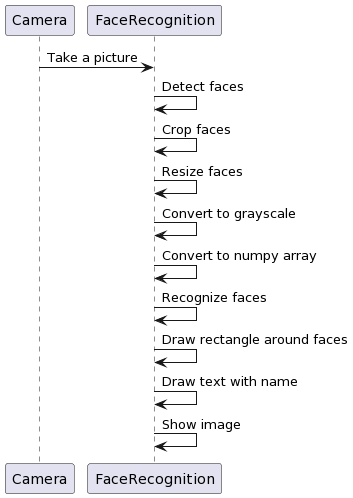
\includegraphics[width=0.5\textwidth]{images/Diagram-1.png}
    \caption{Flowchart of the system}
    \label{fig:flowchart}
\end{figure}

%-------------------------------------------------------------------------

\graphicspath{ {images} }

\section{Team}
    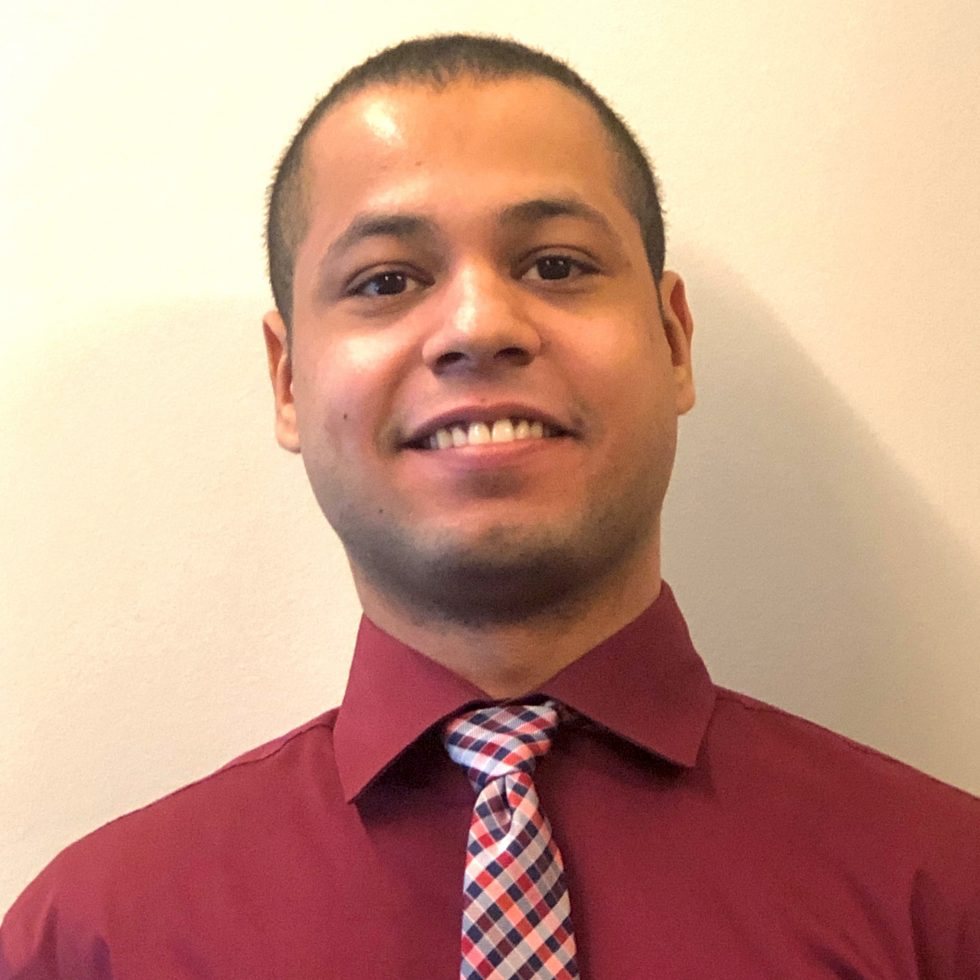
\includegraphics[width=0.1\textwidth]{Murtadha.jpg}\\ \textbf{Murtadha Marzouq}\\ \href{https://webpages.charlotte.edu/mmarzouq/English/Resume.pdf}{\underline{Resume Link}}\\
   \includegraphics[width=0.1\textwidth]{Param.png}\\ \textbf{Param Patel}\\  \href{https://drive.google.com/file/d/13jr45PMGy9iJG0CavpYmuiN5SDwGgygj/view?usp=sharing}{\underline{Resume Link}}\\

\includegraphics[width=0.1\textwidth]{Haochen.png}\\     \textbf{Haochen Ye}\\ \href{https://drive.google.com/file/d/1YOZvJANmngCAai1OxXm28a_7XmKGmpH1/view?usp=sharing}{\underline{Resume Link}}\\

\includegraphics[width=0.1\textwidth]{Sam.png}\\     \textbf{Sam Aldehayyat}\\ \href{https://drive.google.com/file/d/14jBT5AZ_GzdElLh-0LSXzP7AxgjMu0wa/view?usp=sharing}{\underline{Resume Link}}\\

\includegraphics[width=0.1\textwidth]{Yuepei.png}\\     \textbf{Yuepei Yu}\\ \href{https://drive.google.com/file/d/1xcBhl6kxY1gQZsCjADVlJvvDVYBJLoSo/view?usp=sharing}{\underline{Resume Link}}\\

{
    \small
    \bibliographystyle{ieeenat_fullname}
    \bibliography{main}
}

% WARNING: do not forget to delete the supplementary pages from your submission 
% \clearpage
\setcounter{page}{1}
\maketitlesupplementary


\section{Rationale}
\label{sec:rationale}
% 
Having the supplementary compiled together with the main paper means that:
% 
\begin{itemize}
\item The supplementary can back-reference sections of the main paper, for example, we can refer to \cref{sec:intro};
\item The main paper can forward reference sub-sections within the supplementary explicitly (e.g. referring to a particular experiment); 
\item When submitted to arXiv, the supplementary will already included at the end of the paper.
\end{itemize}
% 
To split the supplementary pages from the main paper, you can use \href{https://support.apple.com/en-ca/guide/preview/prvw11793/mac#:~:text=Delete%20a%20page%20from%20a,or%20choose%20Edit%20%3E%20Delete).}{Preview (on macOS)}, \href{https://www.adobe.com/acrobat/how-to/delete-pages-from-pdf.html#:~:text=Choose%20%E2%80%9CTools%E2%80%9D%20%3E%20%E2%80%9COrganize,or%20pages%20from%20the%20file.}{Adobe Acrobat} (on all OSs), as well as \href{https://superuser.com/questions/517986/is-it-possible-to-delete-some-pages-of-a-pdf-document}{command line tools}.

\end{document}
